% Tipus de document
\documentclass[a4paper]{article}
% Utilitzar tota l'amplada de la pàgina
\usepackage{fullpage}
% Extres de LaTex
\usepackage{latexsym}
% Text en utf8
\usepackage{ucs}
\usepackage[utf8x]{inputenc}
% Text generat automàticament en català i partició per síl·labes
\usepackage[catalan]{babel}
% Per afegir imatges
\usepackage{graphicx}

% Autor
\author{Albert Sellarès Torra \texttt{<whats@wekk.net>}\\
        Facultat d'Informàtica de Barcelona,\\
        UPC\\}
%\date{2009}

% Títol de l'article
\title{skd: Rootkit per sistemes operatius UNIX}

% Millora el pdf. Ha de ser l'últim del preàmbul
\usepackage[pdftex,bookmarks,colorlinks,pdfnewwindow]{hyperref}
% \hypersetup{linkcolor=black}

\begin{document}

% Portada
\maketitle
\newpage

\section{Introducció}

Aquest projecte tracta d'implementar una prova de concepte del què seria un rootkit\footnote{rootkit:
Eina o conjunt d'eines que té com a finalitat amagar-se a i amagar altres programes, processos, arxius, 
directoris, ports, etc., per tal que permeti a un intrús accedir al sistema (normalment remotament), 
així com extreure informació.} per a sistemes operatius actuals basats en UNIX.\\ 

Un rootkit és una aplicació pensada per a ser utilitzada com a porta del darrere per tal de
poder accedir i controlar un sistema, i que a més, s'amaga per a no ser descobert.\\

És sabut que existeixen programes fets amb aquesta finalitat, però la majoria d'ells són
per sistemes Windows, no estan públics a la xarxa, estan desfasats i ja no poden ser
usats en els sistemes operatius actuals. A més, els nuclis de sistemes operatius actuals, implementen cada vegada més
proteccions per tal d'evitar que programes com aquests els controlin.

\subsection{Motivació del projecte}

Avui en dia ens veiem immersos en la societat de la informació, un moment en què la
majoria de les empreses i persones intentem adaptar-nos a les noves tecnologies,
moment en què s'intenta digitalitzar tot el què es pot. Qui més qui menys veu que en uns anys tot es veurà gestionat a través de sistemes
d'informació, tot estarà interconnectat entre sí, i s'ha de poder garantir que tots aquests
sistemes, comptin amb un mínim de seguretat.\\


Les implicacions que té estar infectat per un virus estan canviant. Els virus (i en particular
els cavalls de Troia) ja no es fan per molestar a l'usuari, al contrari, un alt percentatge dels
virus tenen com a objectiu principal ocultar-se. Passant desapercebuts, permeten a l'infectant
controlar la nostre màquina podent fer qualsevol cosa en ella com per exemple, apoderar-
se de la nostra compta bancària.\\
Parem-nos a pensar per un moment què passaria si en comptes de què l'infecció estigués
a la nostre màquina, aquesta estigués als servidors on es fan les nostres nòmines, als dels
nostre banc, o a les de qualsevol pàgina de venta d'articles per internet. El perill i la
criticitat, es disparen exponencialment.\\

Des de els inicis de la història els sistemes operatius UNIX han estat al capdavant en els
entorns de servidors, i des de llavors que les grans empreses els utilitzen per a confiar-hi
les seves dades. Avui, i gràcies al boom que ha fet el GNU/Linux i en general el programari lliure(tothom qui més qui
menys té una idea del què és), administradors de sistemes no experimentats acaben
utilitzant sistemes basats en UNIX en el seu lloc de treball. \\
El fet és que actualment moltes empreses utilitzen aquests sistemes operatius (com poden ser
GNU/Linux, BSD, Solaris, etc) per als seus servidors, i són moltes les què s'acaben despreocupant
de la seguretat dels servidors donant com a excusa que un sistema basat amb UNIX és
més segur, i que a més, no hi han virus. A la practica, molta gent que es dedica a
administrar aquestes màquines, no està qualificada, o no compta amb el temps necessari
per a fer-ho del tot bé, i com que les coses aparentment funcionen, es segueix així.
Aquest és el punt on vull arribar. Avui, una persona amb suficients ganes, temps i
coneixements, pot guanyar accés a la majoria de servidors, on un cop accedit, la seva
preocupació principal, és mantenir-ne l'accés.\\

Amb aquest projecte, intento posar de manifest creant una prova del concepte, lo difícil
que pot arribar a ser per un administrador de sistemes adonar-se que ha estat infectat per
un rootkit, lo perillós per a la seguretat del sistema, i lo crua que és la realitat ja que un
intrús pot tenir-ho molt fàcil per a controlar el nostre servidor. \\

\section{Objectiu}

L'objectiu del projecte, és implementar un rootkit per a sistemes basats en UNIX. Tot seguit
es descriu en forma de resum, les característiques en un caire general que el rootkit ha de potenciar. \\

\begin{description}
    \item[Ocultació] Ha de passar el màxim desapercebut en el sistema on estigui
    instal·lat. Per un administrador, ha de ser molt difícil d'adonar-se que el
    sistema ha estat compromès. El rootkit ha d'intentar ocultar al màxim les tasques
    que executa. 

    \item[Accés] Ha de permetre l'accés a la persona que
    l'ha instal·lat. Normalment i per comoditat, aquest accés és remot a través
    d'internet. El rootkit ha de facilitar al màxim aquest accés, havent d'evitar les diferents 
    barreres que hi puguin haver (firewalls, ACLs, etc). 

    \item[Administració] Ha de permetre realitzar tot tipus
    d'accions a la màquina com si d'un usuari vàlid es tractés. Accions com executar
    tasques, editar fitxers, pujar o descarregar-ne, són funcionalitats bàsiques que ens
    ha de permetre efectuar. 

    \item[Permanència] Les màquines s'actualitzen, es paren i s'engeguen. El rootkit ha
    d'intentar no veure's afectat per aquests canvis. 

    \item[Augment de privilegis] Ha de ajudar tant com pugui, a la obtenció de nous
    privilegis. Altres comptes d'usuari, comptes d'altres màquines, comptes de bases de dades, etc.
\end{description}
Cal dir que en la memòria del projecte totes aquestes funcionalitats estaran descrites amb molt més detall. De 
tota manera, podeu contactar amb mi per a aclarir qualsevol dubte. 

\section{Planificació}

La planificació del projecte, és la següent:
\begin{figure}[htp]
    \centering
		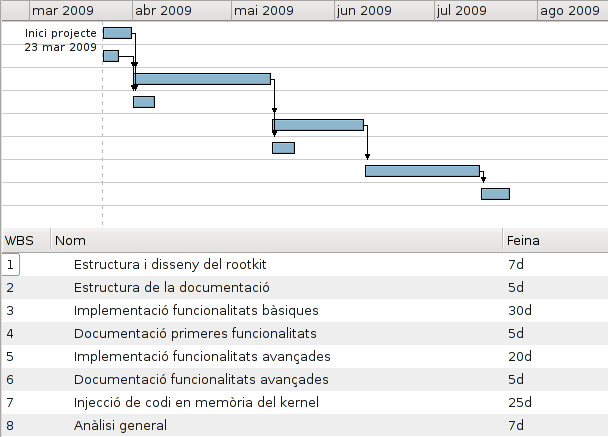
\includegraphics[scale=0.7,keepaspectratio]{primer_gantt.png} 
    \label{fig:gantt}
\end{figure}

Els punts principals d'aquesta planificació, són el fet de no deixar la documentació del projecte pel final,
sinó que fos un punt que s'anés avançant constantment. S'han separat les diferents tasques entre el disseny
i la recerca inicial, la implementació de les seves funcionalitats en dos blocs segons la seva dificultat,
una part del rootkit a nivell de kernel i només per a GNU/Linux, i finalment un anàlisis general per a polir-ho
i homogeneïtzar-ho tot. \\

\section{Què portem fet i què falta?}

A dia d'avui, de la part de la memòria, només falta completar el capítol Solució que és on s'exposen els
detalls tècnics del projecte. \\

Del desenvolupament del rootkit, falten per desenvolupar algunes de les funcionalitats avançades, així com 
algunes de les funcionalitats que inicialment no estaven incloses en ell, però que hem cregut convenient
afegir-les.

\end{document}
